\chapter{Experiment No.3: Semiconductor Detectors}
\section{Description}
\textbf{ExperimentalSetup}
In this part of the experiment we connect semiconductor detectors to a Multi Channel Analyzer (MCA). The signal gets amplified as can be seen in the sketch below:\\
\begin{figure}[h]
\begin{center}
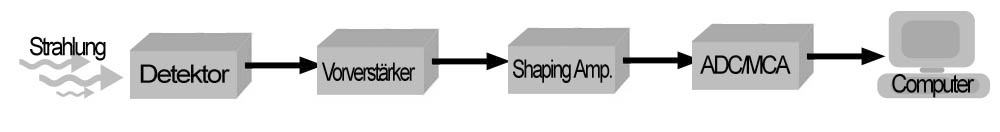
\includegraphics[scale=0.3]{Bilder/Aufbau_V3.png}\caption{Experimental setup. Source: [Ver]}\label{Halbleiterdetektor}
\end{center}
\end{figure}\\
\\
The computer measures the spectra with the help of a program called ADC. We use two different semiconductor detectors: a n-$n^{+}$-silicon-diode and a CdTe-crystal.\\
\\
\large\textbf{Signal curve}
The semiconductor detectors generate a current proportional to the energy of the incoming $\gamma-quanta$. The preamplifier boosts the signal strength. The signal then reaches the shaping amplifier, where it charges a capacitor, which gets discharged with the help of an electric resistance (CR-filter). The signal has to cross two RC-filters afterwards, which damp the increase of the resulting signal. This $CR-(RC)^2-shaping$ creates a voltage peak. The proportionality between the incoming photon energy and the peak is maintained.\\
\\
\section{Analysis}
The spectra of Am-241 and Co-57 with both detectors can be found in the appendix. For the 122,07 keV measured with CdTe, ADC seems to have reached the maximum counts it's capable of displaying. Thus we added the maximum count number to the counts referring to the canals where we think the peak should've been (there was a clearly visible peak, but with the wrong number of counts). Both plots are disclosed. The result looks very reasonable, so we decided to continue calculating with the corrected version. Of course a systematic error occurs this way because we don't know the exact number of maximum counts ADC is capable of displaying. But as the resulting curve looks just as expected, we decided on neglecting that error.\\
We did Gaussian fits at the following energies: 59,5 keV for Am-241, 122,07 keV and 136,47 keV for Co-57. The expectation values of the Gaussian fits allow us to connect the energies mentioned above (the peaks) to certain channel numbers. In the table below the channels referring to certain energies are listed:\\
\\
    \begin{tabular}{rrrrr}
    Detector & Sample & Channel no. & Error & Energy (keV) \\
    Si    & Am-241 & 301,8 & 0,1   & 59,5 \\
          & Co-57 & 623,7 & 0,7   & 122,06 \\
          & Co-57 & 693,9 & 0,1   & 136,47 \\
    CdTe  & Am-241 & 313,8 & 0,2   & 59,5 \\
          & Co-57 & 651,5 & 0,4   & 122,06 \\
          & Co-57 & 728,8 & 0,8   & 136,47 \\
    \end{tabular}%
  \label{tab:addlabel}%
\\
We subtracted 9 from the expectation values for CdTe as the first 9 rows in Origin were occupied with the settings. \\
Of course the channel numbers can only be integers. Still, here we decided to use the exact values with their errors as we wanted to make the energy calibrations as good as possible. The linear fits for the calibrations can be seen below:\\
\begin{figure}[h]
\begin{center}
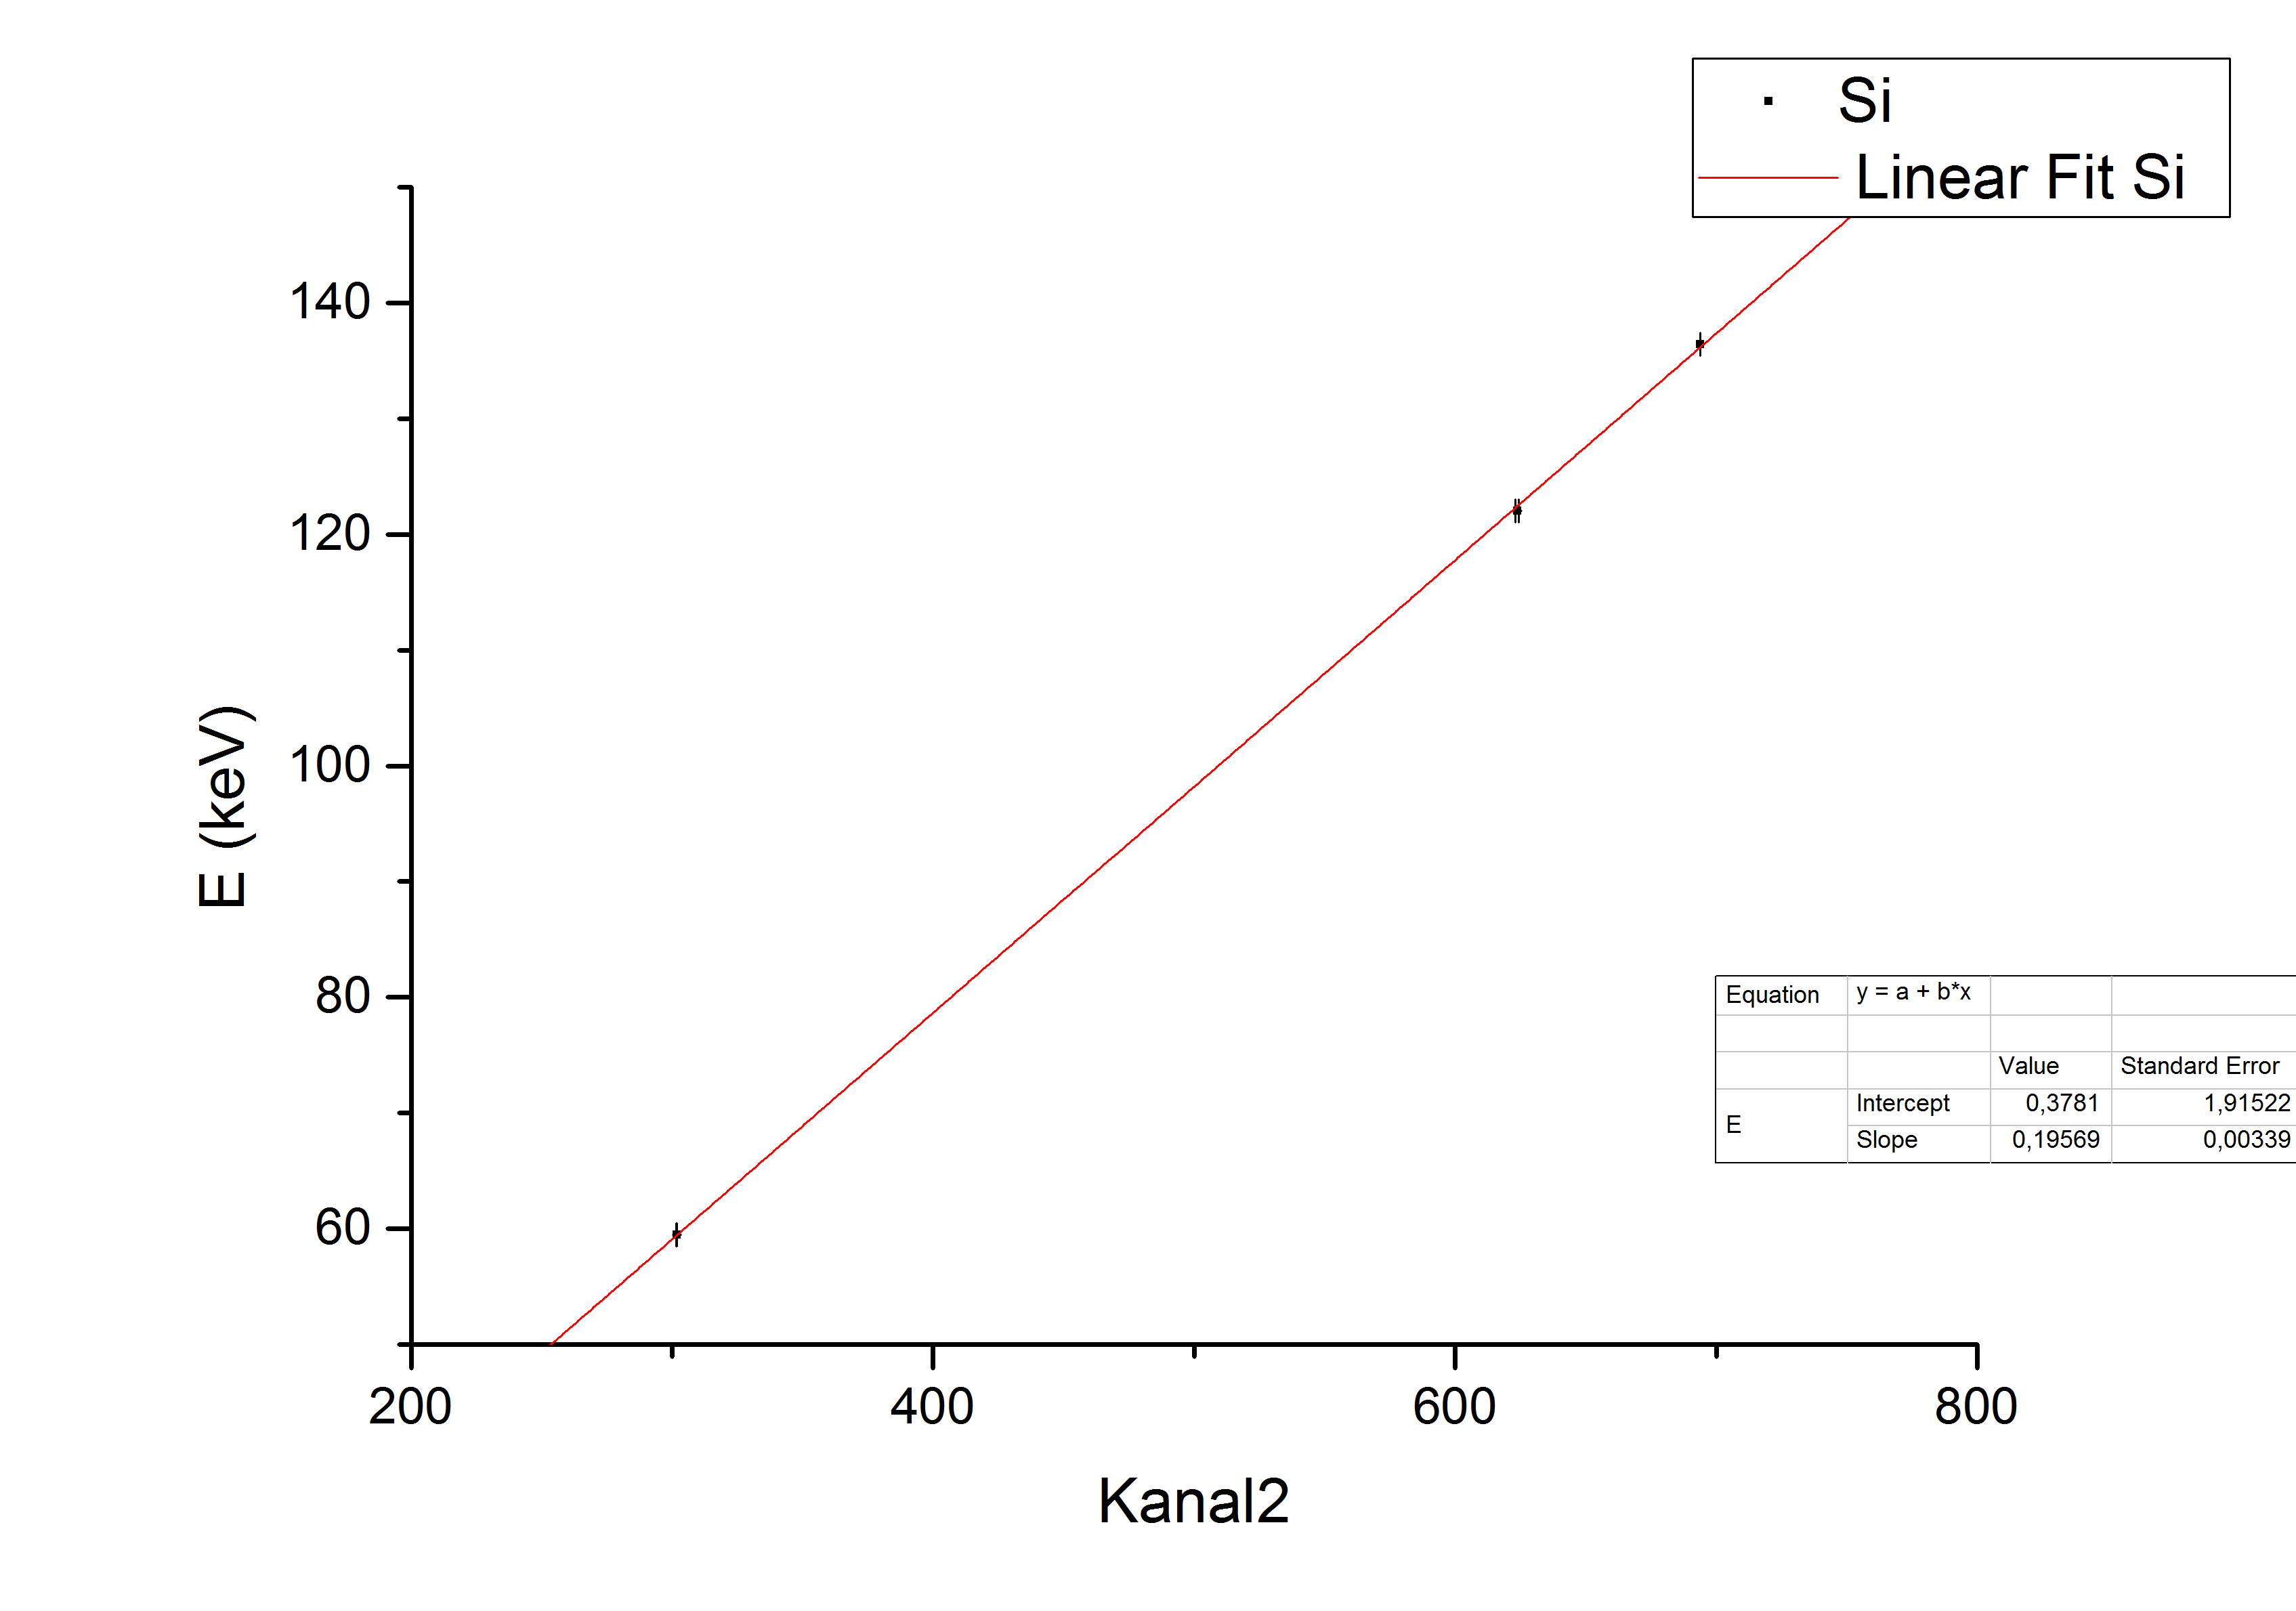
\includegraphics[scale=0.35]{Bilder/linfit_Si.png}\caption{Linear fit silicon}\label{linfit_Si}
\end{center}
\end{figure}\\
\begin{figure}[h]
\begin{center}
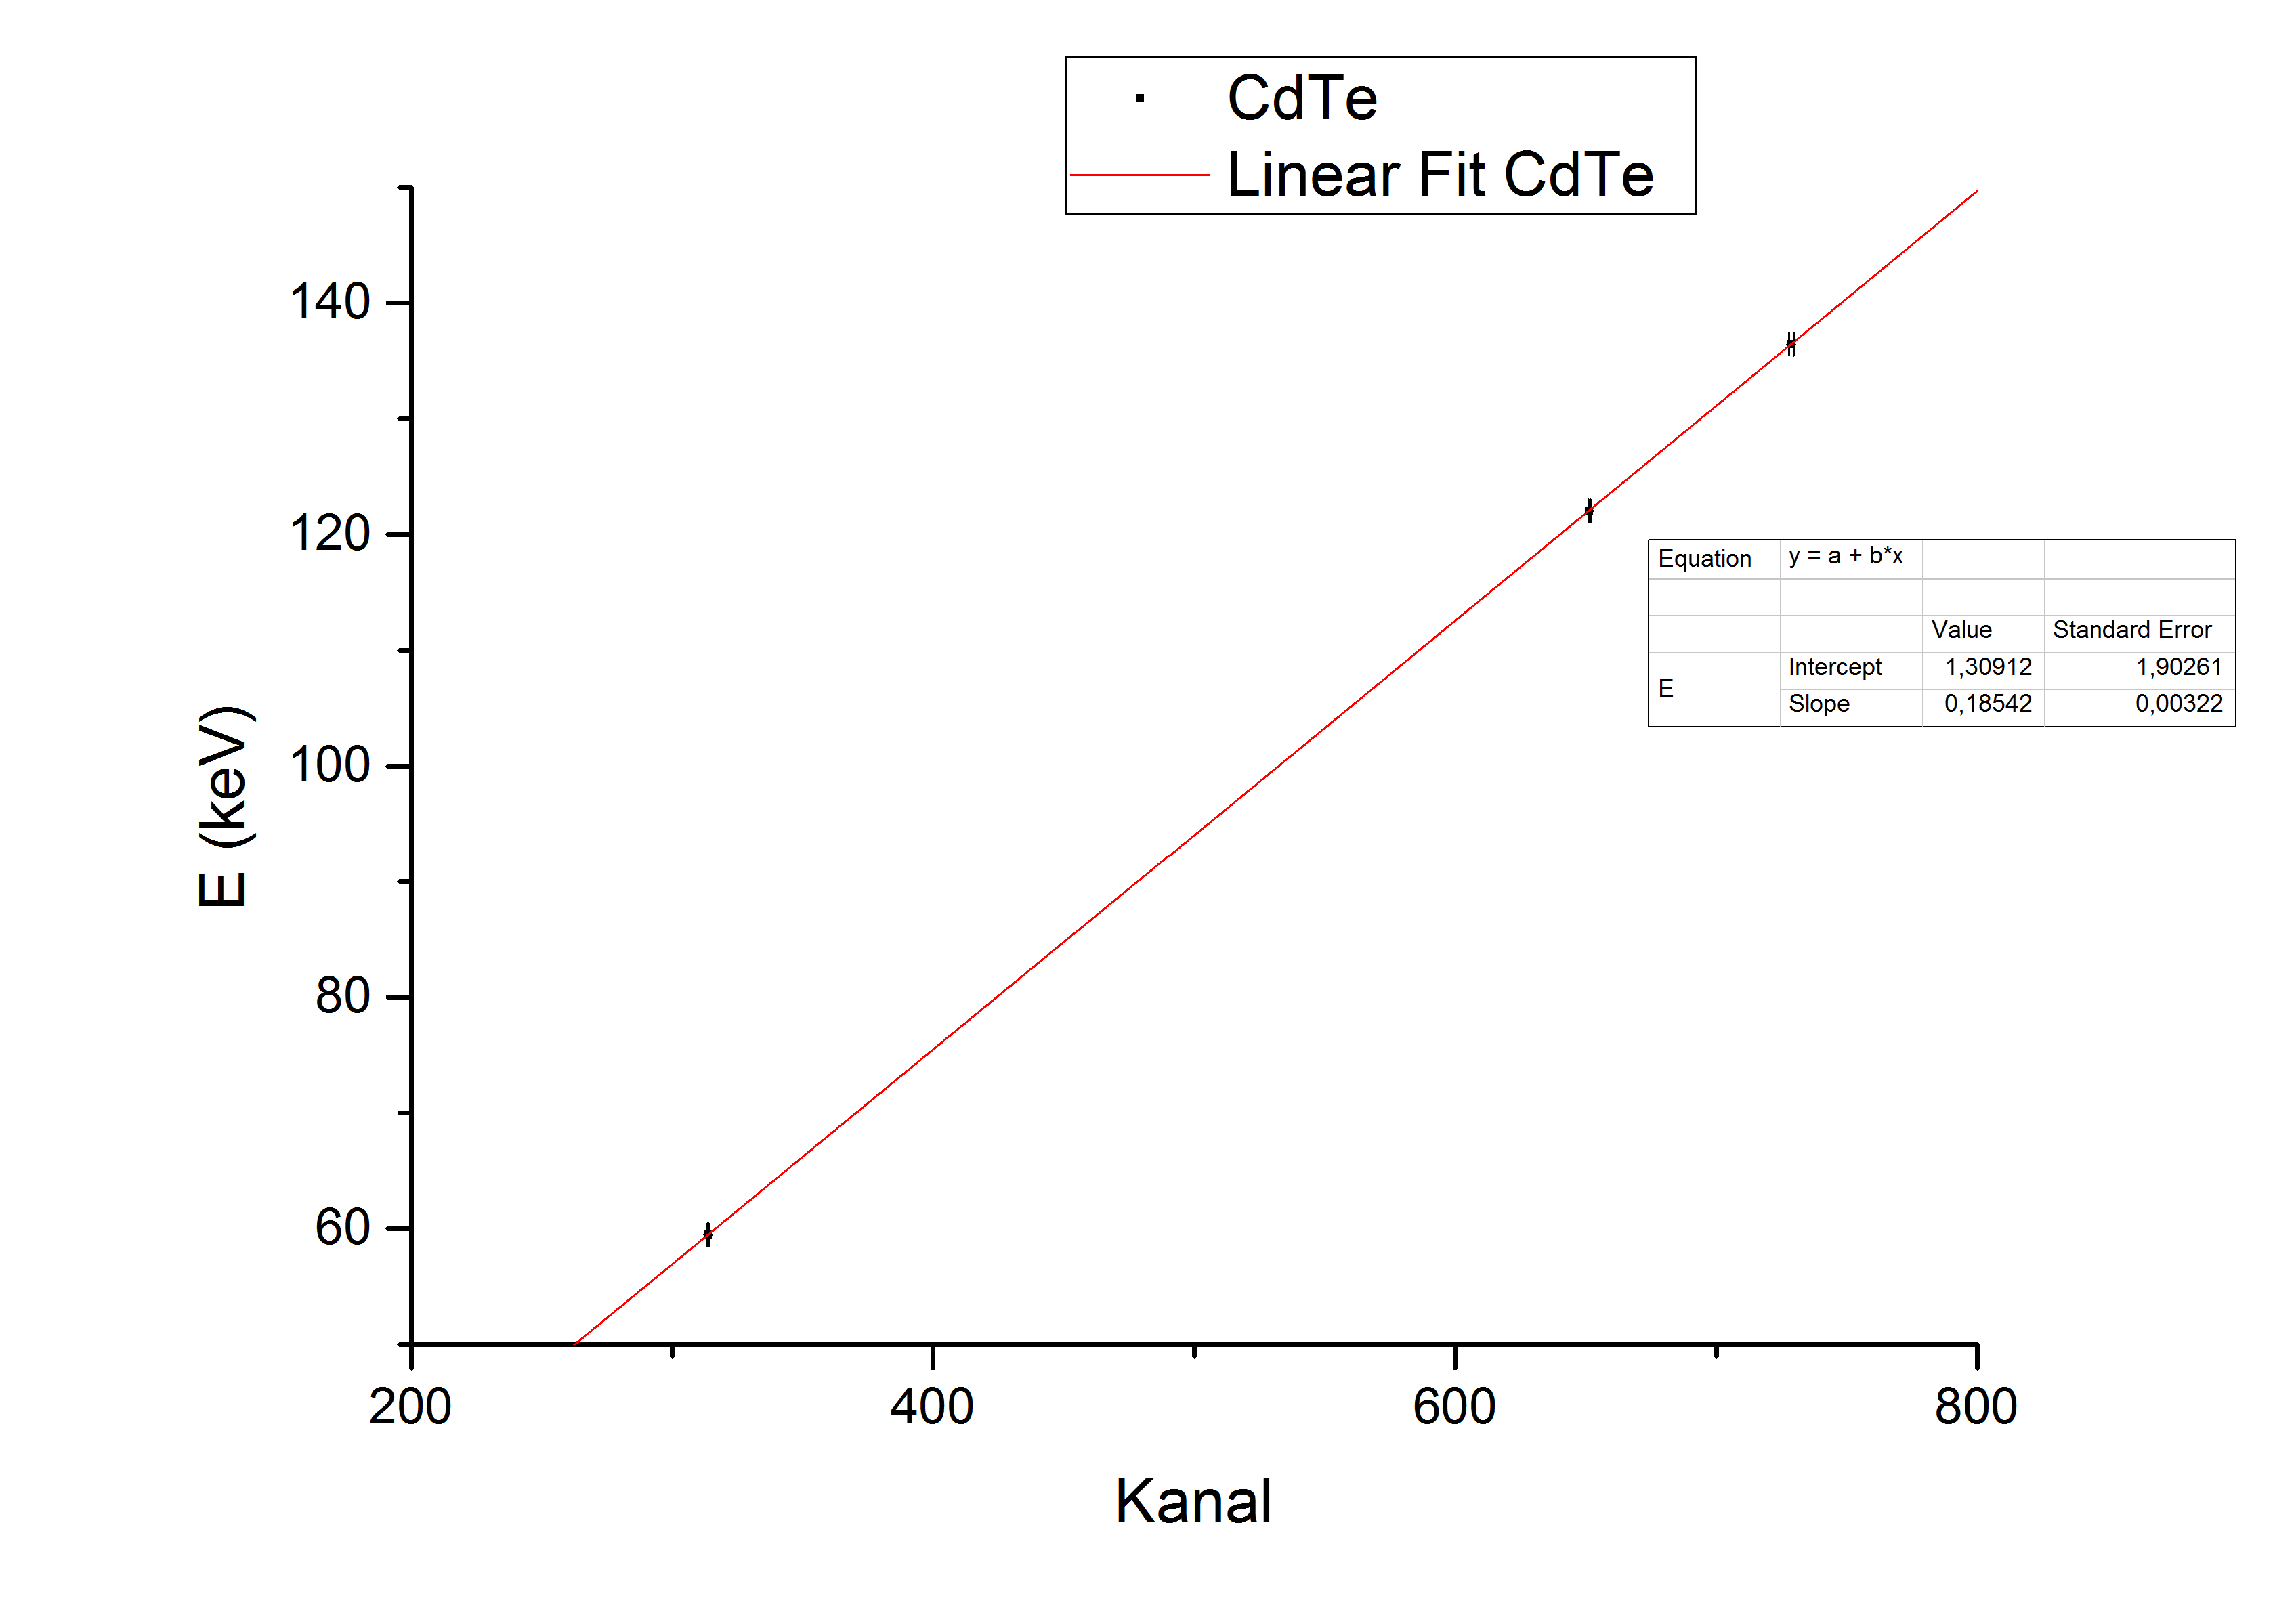
\includegraphics[scale=0.35]{Bilder/linfit_CdTe.png}\caption{Linear fit CdTe}\label{linfit_CdTe}
\end{center}
\end{figure}\\
\\
The energy calibration did obviously work well, as all the measured points can be connected very well with a linear fit.\\
\\
The goal of the experiment is now to compare the absorption probabilities and the energy resolutions of the Si- and CdTe-detector.\\
\\
\textbf{Absorption probability}\\
\\
To determine the ratio of the absorption probabilities of the detectors, we need a value A of the Gaussian fits, which is determined directly when doing the fit and tells us how many incidents occurred. It is $A=amplitude*\sqrt{2*\pi*\sigma^2}$. This value is divided by the surface area of the respective semiconductor detector, because this area is different for Si and CdTe $(a_{Si}=100mm^2, a_{CdTe}=23mm^2)$.\\
\\
It is:\\
\\
$\frac{A_{Si}/a_{Si}}{A_{CdTe}/a_{CdTe}}=\frac{Abs_{Si}}{Abs_{CdTe}}=R$\\
\\
$\Rightarrow$ The error is:\\
$s_{R}=\frac{Abs_{Si}}{Abs_{CdTe}}*\sqrt{(\frac{s_{A_{Si}}}{A_{Si}})^2+(\frac{s_{A_{CdTe}}}{A_{CdTe}})^2}$\\
\\
The results we got are in the table below:\\
\begin{table}[htbp]
  \centering
  \caption{Results}
    \begin{tabular}{rrrr}
    Energy in keV & Ratio R & Error s\_R & Literature value \\
    59,5  & 0,031 & 0,002 & 0,014 \\
    122,06 & 0,00023 & 0,00006 & 0,0183 \\
    136,47 & 0,000013 & 0,000009 & 0,02 \\
    \end{tabular}%
  \label{tab:addlabel}%
\end{table}%\\
\\
Obviously all our values, especially the ones for Co-57, are not even close to their respective literature values. This is not surprising regarding the fact that for silicon the spread for the peaks is just too large to do a proper Gaussian fit (see appendix). For 136,47 keV one needs some imagination to even see a peak at all: we'd rather say that what we measured there cannot really be called a peak. \\
There can be various causes for why our results aren't good: there's a systematic error as we neglect absorption in the epoxy layer. Also, because of the few counts for the 136,47 keV-peak (for Si) the noise is high, because of which the error of the Gaussian should be much larger than we actually determined it to be. Another cause could be an offset in the sample mounting: when changing the detectors, we had to remove the sample and put it back on, so that it's possible that there's a systematic error because we did not put back the sample to its former spot. It's also possible that there's some sort of problem with the sample or the electronics.\\
\\
\textbf{Energy resolution}\\
We can determine the energy resolution RER(E) of the detectors using the half-power width of the peaks. For our calculations we used the following formula:\\
\\
$RER(E)=\frac{FWHM(E)}{E} \approx 2,35\frac{\sigma_{E}}{E}$\\
\\
Because it is $E=a+b*channel$, we get the following:\\
\\$RER(E)=2,35\frac{\sqrt{s_{a}^2+channel^2*s_{b}^2+b^2*\sigma_{channel}^2}}{E}$\\
\\
$\Rightarrow s_{RER(E)}=RER(E)\frac{b^2*\sigma_{channel}*\sigma_{\sigma_{channel}}}{\sigma(E)}}$\\
This way we get the following for the energy resolution:\\
\\
\\
\\
\\
\\
\\
\\
\\
\\
\caption{Energy resolutions}
    \begin{tabular}{rrrr}
    Detector & Energy in keV & RER[E]  & s\_RER[E] \\
    Si    & 59,5  & 0,121 & 0,003 \\
          & 122,06 & 0,068 & 0,007 \\
          & 136,47 & 0,05229 & 0,00005 \\
    CdTe  & 59,5  & 0,118  & 0,006 \\
          & 122,06 & 0,060 & 0,005 \\
          & 136,47 & 0,07  & 0,04 \\
    \end{tabular}%
  \label{tab:addlabel}%
\\
Although we don't have literature values given here, obviously because of the errors listed above these won't be good results. Still, at least for Si we could prove a general tendency: the larger the energy is, the better is the resolution. Obviously the error for the third value of the Si-detector is way too low, which is due to the fact that there is not really a peak, making the Gaussian fit having a too small width.





